\documentclass[12pt]{report}

\usepackage[english]{babel}
\usepackage[utf8x]{inputenc}
\usepackage{amsmath}
\usepackage{graphicx}
\usepackage{multirow}
\usepackage[hypcap]{caption}
\usepackage{setspace} 
\usepackage{float}

\title{Lab 1: Tension Test of Steels}
\author{Zachary Tschirhart \\
	\small \\
        \small EID: zst75 \\
	\small Department of Aerospace Engineering and Engineering Mechanics \\
	\small \textbf{ASE 324L (Mon 2:00-5:00)} \\
	\small Unique: 13740}

\date{January 27, 2014}


\begin{document}
\maketitle

\begin{abstract}
When comparing hot and cold rolled steel, there are significant differences between the two. By cold rolling steel, the structure of the atoms are realigned and form a more unified structure. This realigning will make the metal more brittle and increase the strength, but reduce the overall toughness. This is intuitive since the metal is already being deformed and has already absorbed some energy to deform it. The other aspect observed in this lab was the difference in measurements taken and what sources of error occurred. One source of error that occurred was the large discrepancy between the measured results and theoretical. This was mainly due to the non-ideal formation of materials worked with. 
\end{abstract}


\tableofcontents
\pagebreak

\setcounter{secnumdepth}{0}



\section{Introduction}
\doublespacing

This lab had two tension tests performed, one on hot rolled steel and the other on cold rolled steel. The purpose was to demonstrate the effect of such a load on each of these specimen and to allow for students to analyze the collected data. The performed analysis will provide for a better understanding of terms used when characterizing materials, more specifically, 1020 grade steels.   

\section{Experimental and Data Reduction Procedures}

The apparatus used to test each of these specimen was an electromechanical test-machine that had electric motors controlling screws that move a cross-head. The cross-head gripped onto the specimen on each side. This machine applies a ramp loading to the specimen, which allows for the recording the change in length and diameter change by using extensometers. The extensometers are placed directly on the specimen before loading occurs and stay attached right up the fracture point. 

The loading of the specimen is caused by the motors turning the screws attached to the cross-head. This causes a tensile force in the specimen enclosed in the grips. This force was captured by the test machine and given as a voltage. Each of the extensometers also output as a voltage and is converted into a physical measurement by using a calibration number. The three calibration numbers used were for load (2 lb/v), \% strain (3 \%/v), and radial displacement (4 inch/v). These calibration numbers were then multiplied by the output voltages in order to get the physical measurement. 

In order to get the stress values for the specimen, the following equation needed to be used to convert from the load. 

\begin{equation}
        \sigma = \frac{4P}{\pi d_0^2}
	\label{equation:equation1}
\end{equation}

Where P is the load, and \(d_0\) is the original diameter of the specimen. 

\section{Results and Discussion}
\doublespacing

Over the course of this lab, both cold and hot rolled steel were tested for effects of applying a force causing elongation and ultimatly breaking. While running these experiments, data was collected and the following results are discussed below.

\begin{figure}[H]
	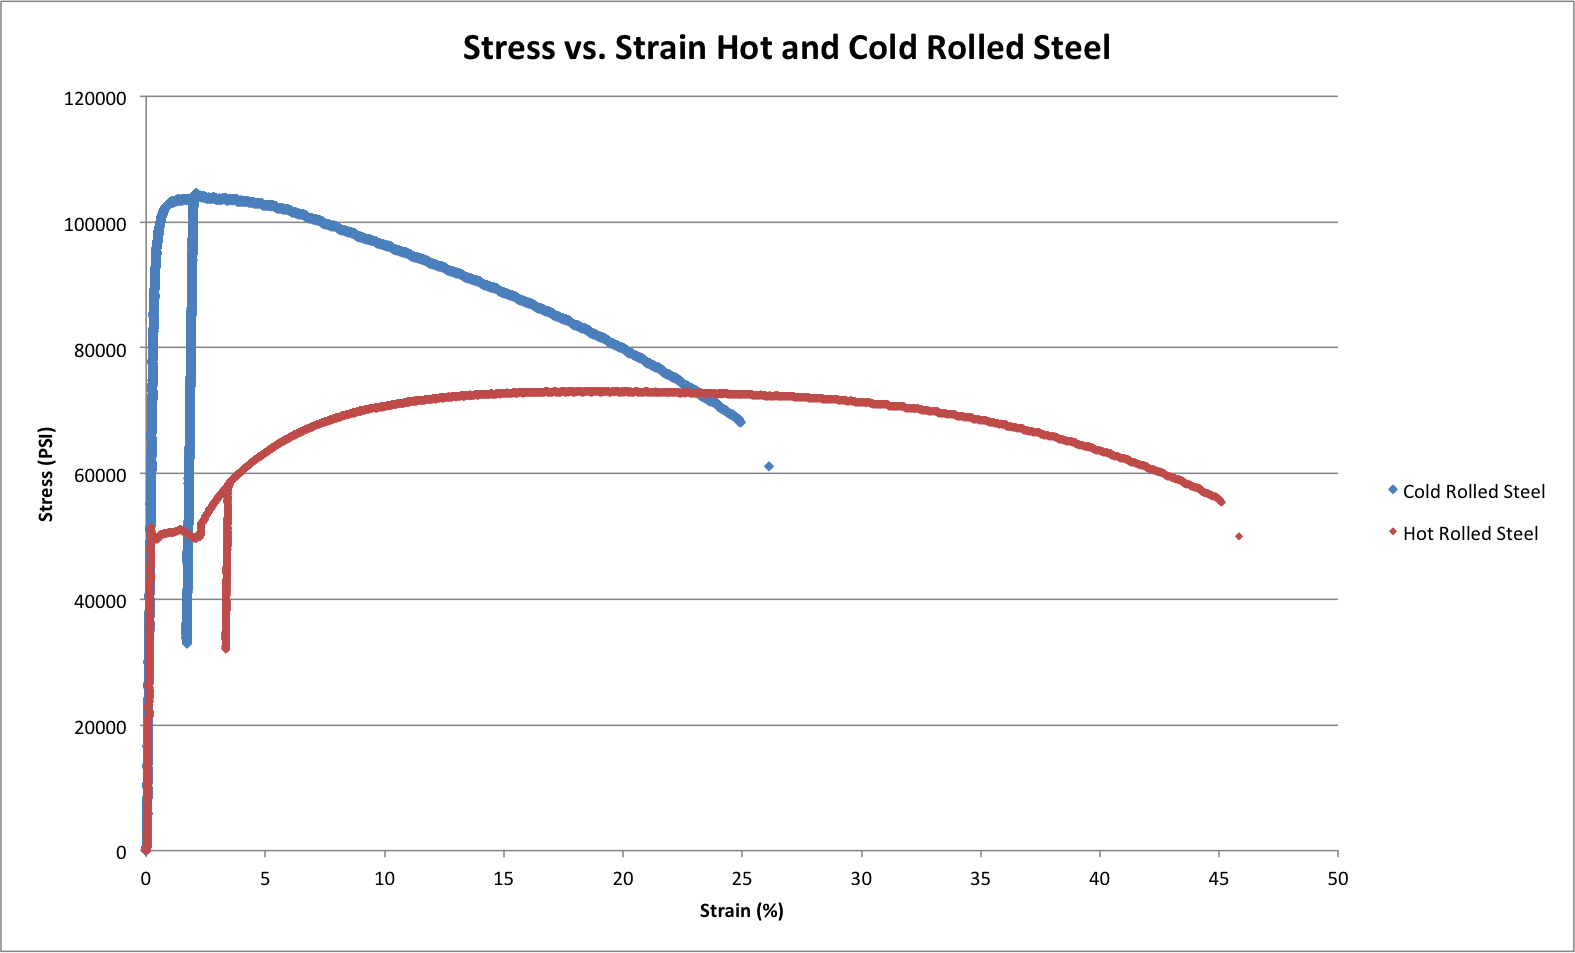
\includegraphics[width=1\textwidth]{stress_vs_strain.png}
	\caption{Engineering stress vs. strain for Hot Rolled Steel}
	\label{fig:Figure1}
\end{figure}



\begin{figure}[H]
	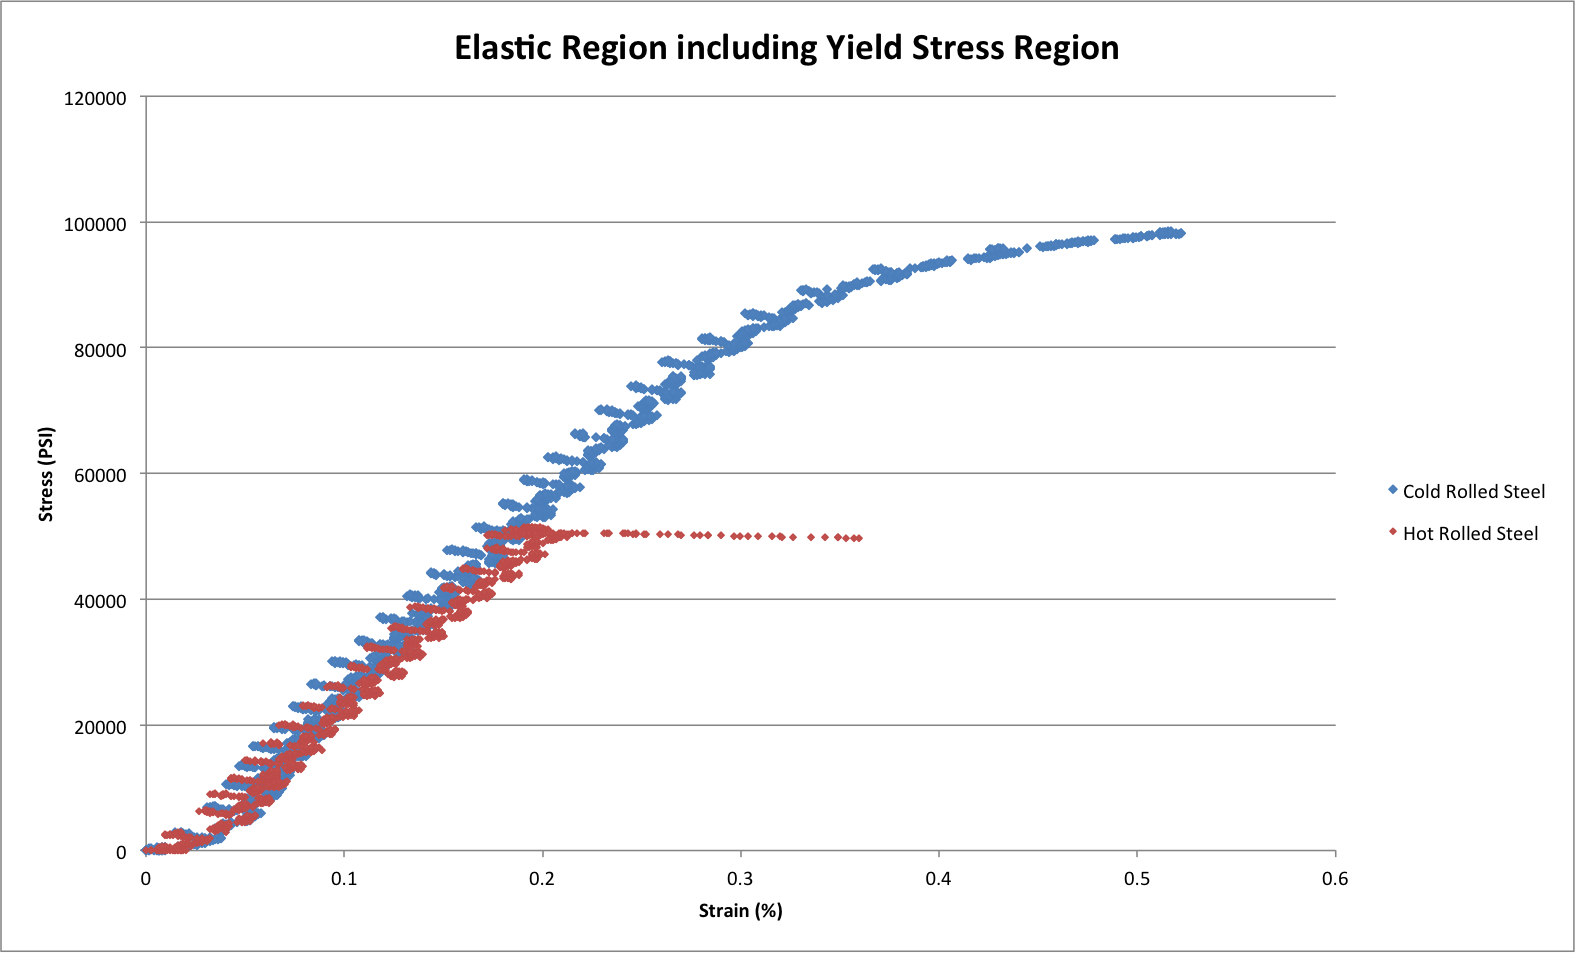
\includegraphics[width=1\textwidth]{elastic_region.png}
	\caption{Engineering stress vs. strain elastic region for Hot Rolled Steel}
	\label{fig:Figure2}
\end{figure}

The elastic region of both specimens are seen on figure 2 where the differences between the two can be observed quite easily. In both cases, a clear linear relationship between stress and strain can be seen, but in the hot rolled steel case the yield stress is much lower than the cold rolled steel. 

\begin{figure}[H]
	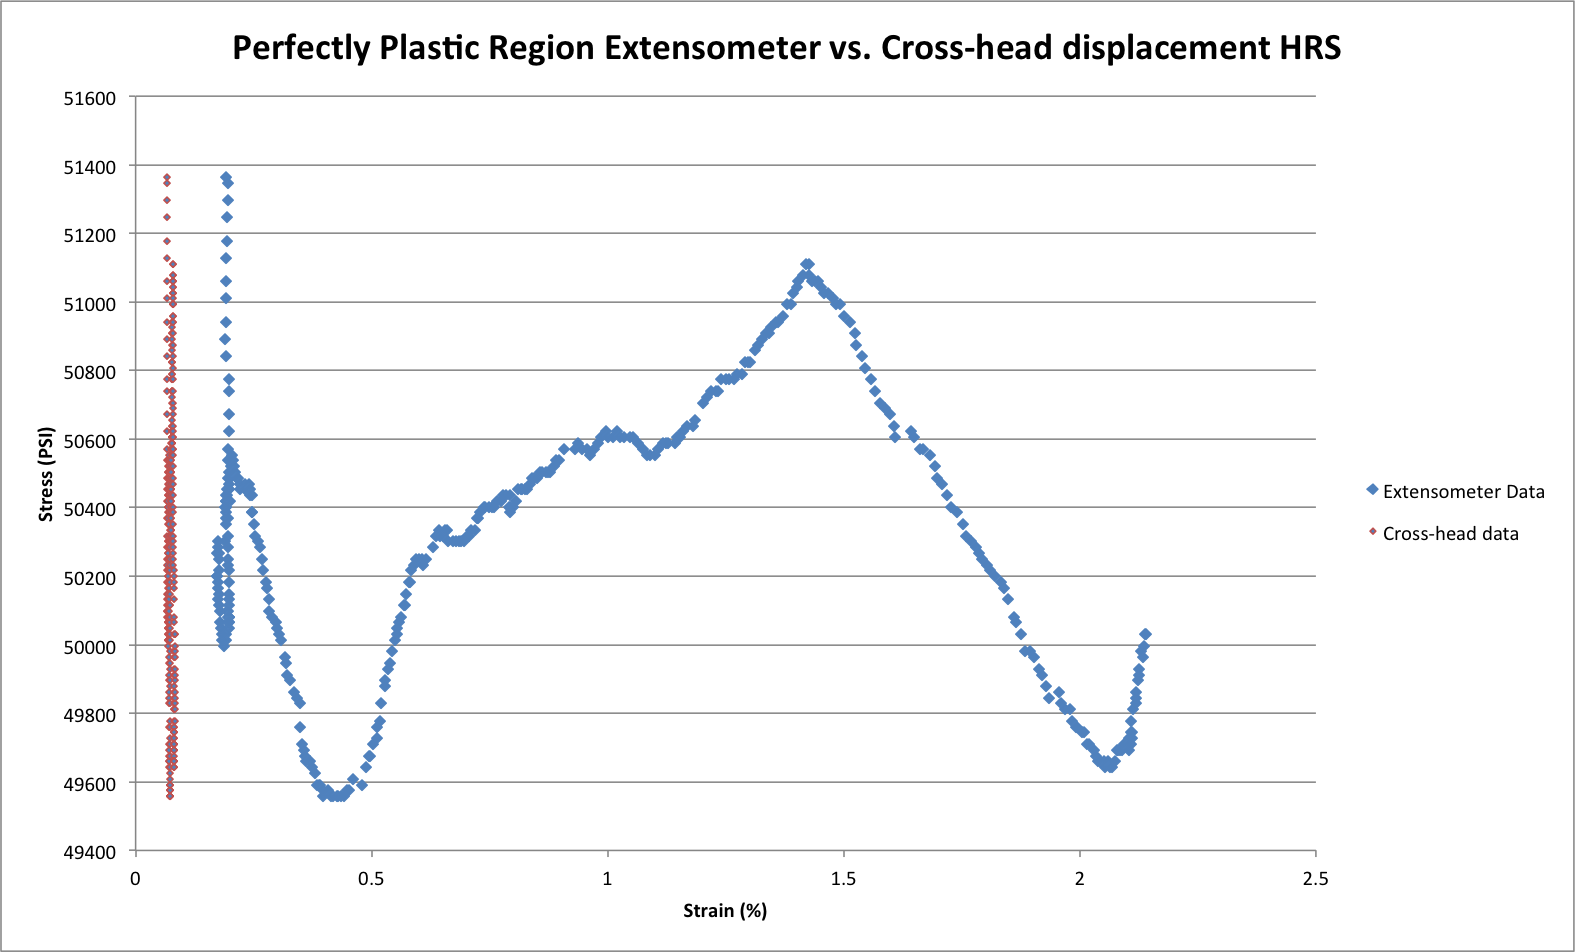
\includegraphics[width=1\textwidth]{extensometer_vs_crosshead_HRS.png}
	\caption{Engineering stress vs. strain comparing Extensometer and Cross-head Displacement data for Hot Rolled Steel}
	\label{fig:Figure3}
\end{figure}

\begin{figure}[H]
	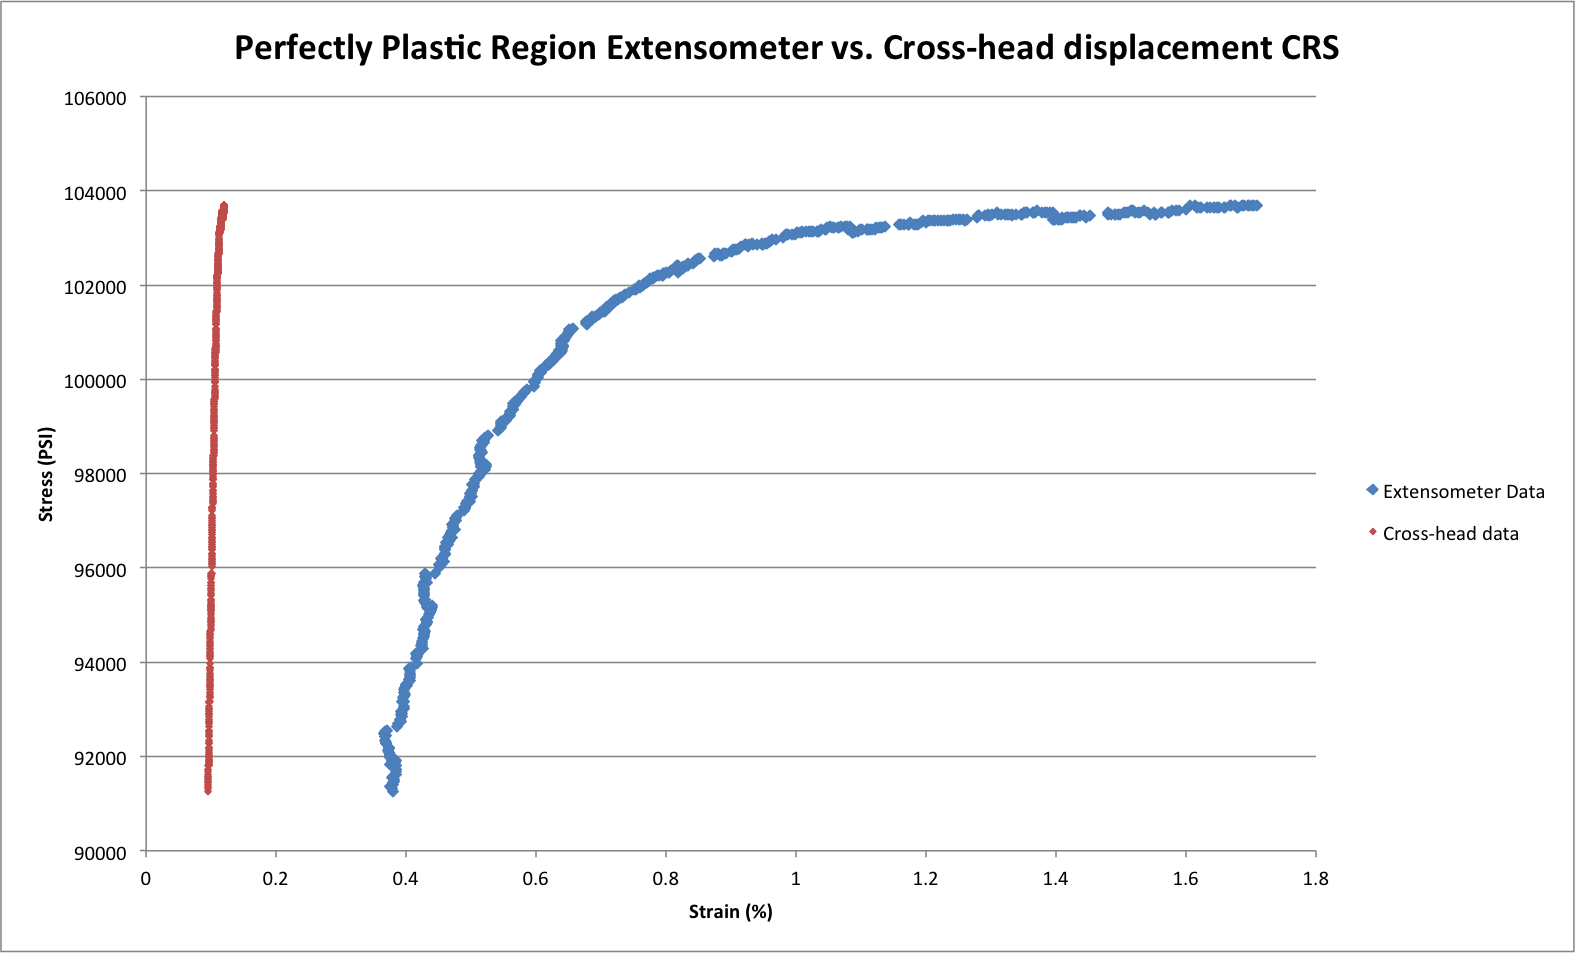
\includegraphics[width=1\textwidth]{extensometer_vs_crosshead_CRS.png}
	\caption{Engineering stress vs. strain comparing Extensometer and Cross-head Displacement data for Cold Rolled Steel}
	\label{fig:Figure4}
\end{figure}

As can be seen in figures 3 and 4, the cross-head computed engineering strain is much less exagerated than the extensometer data. This difference arises because of the range at which each device is measuring strain/elongation. The extensometer is measuring a smaller range and is more sensitive to changes, whereas the cross-head extension measurement is not.

As seen in figure 2, the concept of elastic behavior can be defined as the region in an engineering stress-strain diagram where the relationship between the two is linear. This stress-strain diagram is of a speciman under tensile, uniaxial loading. For a more intuitive definition, the linear elastic behavior is when the hot or cold rolled steel is elongated without permanent deformation. 

Hooke's law for uniaxial loaded members can be summed up in two well known equations:

\begin{equation}
        \varepsilon = \frac{\sigma}{E}
	\label{equation:youngmodulus}
\end{equation}

\begin{equation}
	\varepsilon' = -\nu \varepsilon
	\label{equation:poissonsratio}
\end{equation}

Where \(\sigma\) is the stress, E is the Young's modulus, \(\nu\) is the Poisson's Ratio, \(\varepsilon\) is the axial strain, and the \(\varepsilon\)' is the radial strain.These equations help characterize materials by defining Young's modulus and Poisson's Ratio for materials under a load within the linear elastic region. 

Using the equations above, the Young's modulus and Poisson's Ratio for both hard and cold rolled steel can be found. For the hot rolled steel scenario, the Young's modulus was 247331.58 psi and the Poisson's Ratio was 0.000001. As for cold rolled steel, the Young's modulus was 266175.96 psi and 0.003 for Poisson's Ratio. All of these numbers seem to be two orders of magnitude smaller than the standard values for these materials. This error may have come from incorrect calibration constants or other human errors. The most likely case is due to the impurities and other differences than the ideal material. In the case of the hot rolled steel, the value seemed very different, most likely due to other human factors.

When talking about the elastic region, the proportional limit is the edge of that linear range, also known as the elastic limit for many metals. The yield strength is also very similar to the elastic limit, where it is the practical value that engineers use to specify the load limit before the material starts permanent deformation. The upper and lower yield points for the hot rolled steel were 50132.0 psi and 48393.4 psi, respectively. The 0.2\% offset yield strength for the cold rolled steel was 98085.6 psi. The Poisson's Ratio of each of these materials in the plastic region were 0.0048 for hot rolled steel and 0.0052 for cold rolled steel.

The next region in the stress-strain diagram after the plastic section is strain hardening. Strain hardening is a non-linear region where there is an increase of hardness and strength caused by plastic deformation. Each of these materials went through this state in the stress-strain diagram and an power equation was able to be fitted to the data. The exponent for the cold rolled steel case was 0.1141 while the hot rolled case was a little higher around 0.1732.

At the edge of the strain hardening region in the engineering stress-strain diagram, the ultimate strength of a material is seen. This is known as the hardest stress developed in the material before it breaks. The ultimate strength for the hot rolled steel was 72919.28 psi and for the cold rolled steel it was 104443.92 psi.

In the stress-strain diagram after the material starts to deform in the strain hardening region, necking in the material starts to form, reducing the diameter of the specimen. In the hot rolled steel case, necking occurred in the range of both extensometers and can be seen in figure 1 at the start of strain hardening. In the cold rolled steel case, the necking occurred outside of both extensometers measurement ranges, so the data wasn't recorded in this case. Since the necking did occur outside of the measurement range, this could also be the cause of some error when plotting and figuring any plastic region calculations. If the stress-strain diagram did take this change in diameter into consideration, then the plot would look different after the material moved out of the perfect plasticity region. The differences can be seen in figure 5, where the dotted line indicates the true stress-strain diagram and the solid line indicates the engineering stress-strain diagram. This deviation is the sole result of taking into account the necking diameter when running the experiment.

\begin{figure}[H]
	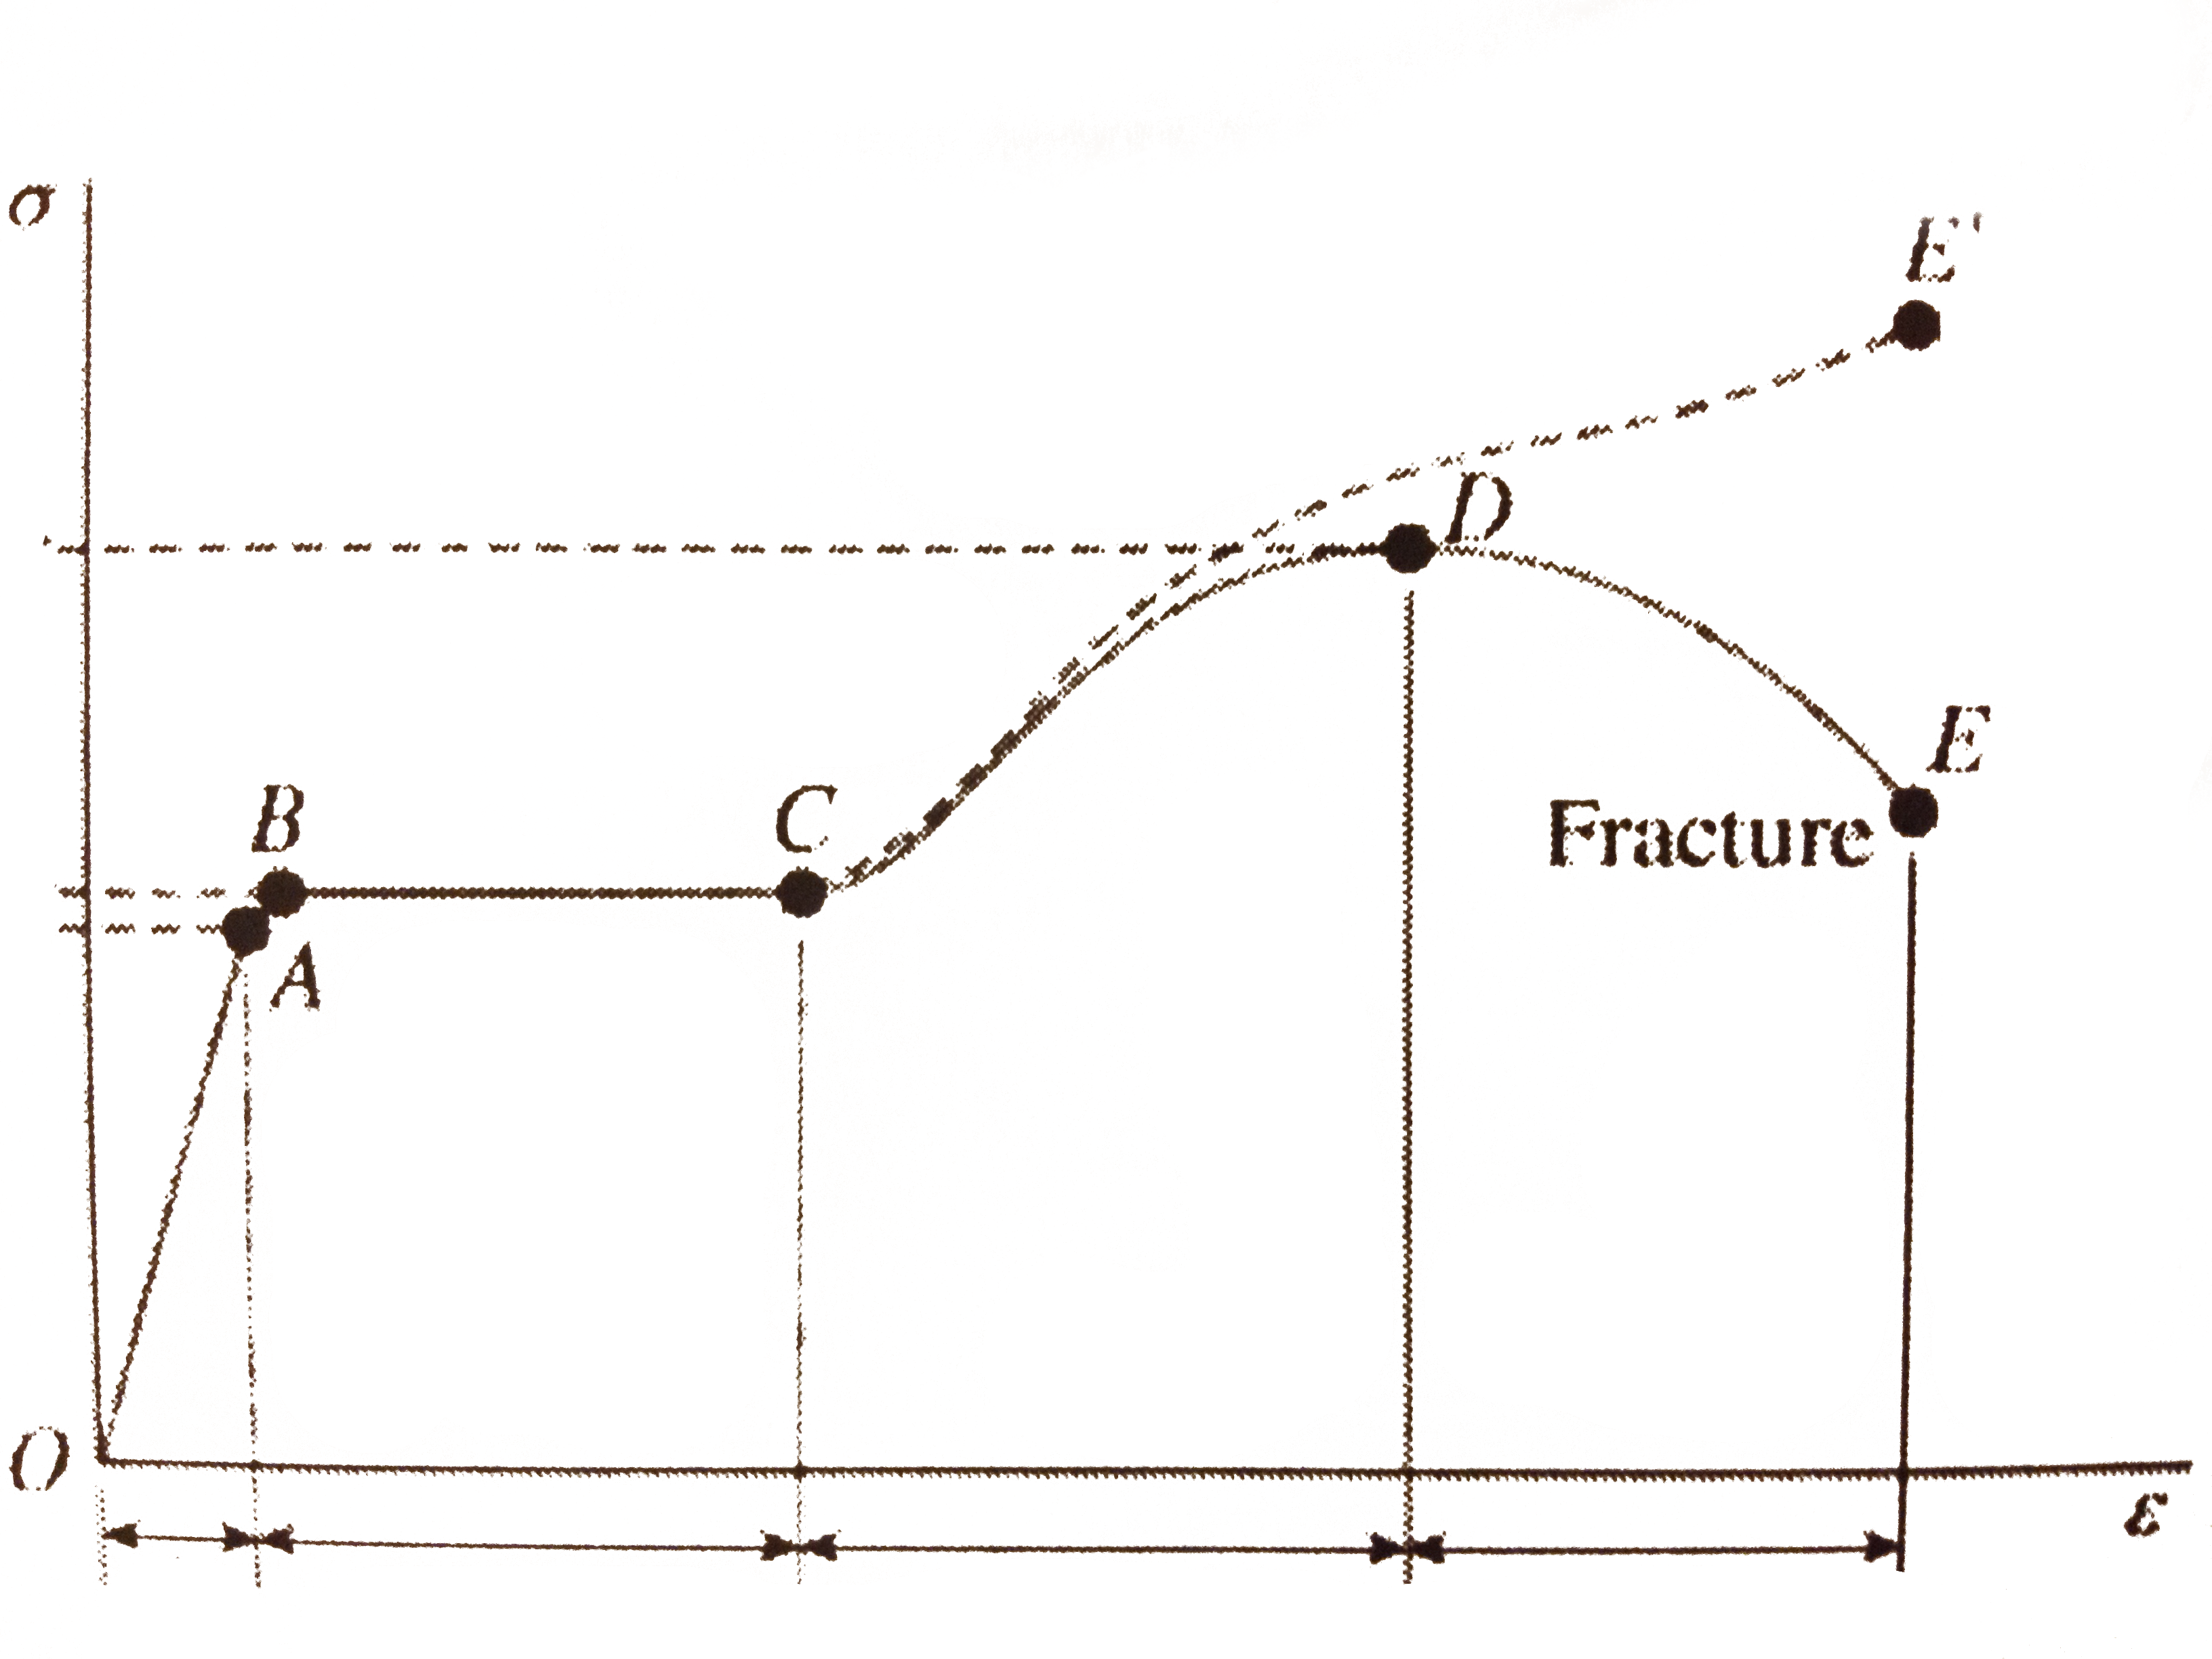
\includegraphics[width=1\textwidth]{true_stress_vs_strain.png}
	\caption{Engineering and True Stress versus Strain diagram [2]}
	\label{fig:Figure5}
\end{figure}

Ductility is the measure of a material's ability to plasticly deform without breaking. This can be measured in several ways; one way is to look at the axial strain at the point of failure on the stress-strain diagrams, and to calculate it by using the original length or area of the specimen and comparing it to the final length or area.

\begin{equation}
        \epsilon_f = \frac{L_f - L_0}{L_0}
	\label{equation:duclength}
\end{equation}

\begin{equation}
	\epsilon_f = \frac{A_0 - A_f}{A_0}
	\label{equation:ducarea}
\end{equation}

Where \(A_0\) is the original area, \(A_f\) is the final area, \(L_0\) is the original length, and \(L_f\) is the final length. Unfortunately, in each experimented case, the extensometer was disconnected before the fracture occurred. The ductility of the hot rolled steel using the area of the specimen was 0.629 and using the length it was 0.258. In the case of cold rolled steel when using area to calculate the ductility, it came out to 0.492 and when using length it was 0.145. 

The difference between the measured length between the extensometer, cross-head displacement, and the marks placed on the specimen before put under a load for each material can be seen in figure 6.
\\
\begin{figure}[H]
    \begin{tabular}{ | l | l | l | l |}
    \hline
    Material & Extensometer (in) & Cross-head disp. (in) & Gage marks (in) \\ \hline
    Hot rolled steel & 0.015 & 0.879 & 0.516 \\ \hline
    Cold rolled steel & 0.015 & 0.475 & 0.290 \\ \hline
    \end{tabular}
    \caption{Table of length changes when measured using three different methods}
\end{figure}\\

The differences between all of the measurements are most likely due to the accuracy of each device. In the case of the extensometer reading, this is can again be attributed to an incorrect calibration value. 

The toughness of a material is determined by integrating the engineering stress-strain curve from the start to when the material fractures. This measurement is to help characterize how much energy the material can absorb before fracturing. By integrating the three sections independently and summing them, the toughness of hot rolled steel is 886317.62 psi while for cold rolled it was 659311.24 psi. 

The apparent similarities between the two rolled steels are small besides the curve after the plastic region. The number of differences are large by comparison, for example the plastic region of the hot rolled steel has a flat section versus the cold rolled steel that has almost no apparent plastic region. The other large difference is the level of stress. 

\section{Conclusion}
\doublespacing
In conclusion, it is clear that the difference between hot and cold rolled steel are apparent in many ways. Putting each specimen under the same loading conditions and recording the changes using several methods and devices. All of the different measurements were different in several ways, but each gave a good indication of what the materials properties were. Overall it seems that cold rolling steel increases the strength, but reduces toughness when compared to hot rolled steel. 




\begin{thebibliography}{0}
\bibitem{notes} {\em ASE 324L Lab manual : The University of Texas at Austin Department of Aerospace Engineering}  2014.
\bibitem{notes} {\em ASE 324L Lecture 2 : The University of Texas at Austin Department of Aerospace Engineering}  2014.
\end{thebibliography}
\addcontentsline{toc}{section}{Bibliography}


\end{document}
